\documentclass[../main.tex]{subfiles}

\begin{document}

\chapter{Формулювання та аналіз вимог до багтрекеру}

\section{Формулювання та аналіз вимог}

\subsection{Формулювання вимог}

Розглянувши існуючі на цей час програмні продукти для багтрекінгу, проаналізувавши їх, та виявивши як позитивні так і негативні їх сторони, можна сформулювати задачі розробки. В узагальненому вигляді такою задачею є створення програмного комплексу, що буде забезпечувати можливість легкого розгортання, підтримки та модифікації системи, а також надання публічного API для спілкування з клієнтами для будь-яких платформ.

При проектуванні програмного продукту необхідно забезпечити наступні можливості:
\begin{enumerate}
    \item Авторизація за допомогою внутрішнього аккаунта.
    \item Можливість управління проектами та їх учасниками.
    \item Можливість управління правами учасників проекту.
    \item Збереження даних щодо проблем/пропозицій.
    \item Можливість прикріплення додаткових артефактів до кожного звіту.
    \item Можливість написання клієнту під будь-яку платформу завдяки вікористанню розподіленої моделі взаємодії.
    \item Синхронізація між пристроями користувачів.
    \item Інтерфейсна частина клієнтського додатку повинна забезпечувати відображення списків проектів, проблем/пропозицій, інформації про проблему, додатків до проблеми.
\end{enumerate}

\subsection{Аналіз вимог}

\subsubsection{Авторизація за допомогою внутрішнього аккаунта}
Для того щоб багтрекінгова система працювала кожний користувач повинен мати свій обліковий запис в базі даних. Серед варіантів реалізації авторизації є два основних підходи: використання власної бази облікових записів або використання стороннього сервісу облікових записів. Реалізація підходу з використанням стороннього сервісу авторизації має декілька проблем:
\begin{itemize}
    \item Можливість зміни механізму авторизації третьою стороною (що автоматично унеможливлює авторизацію)
    \item Відсутність можливості контролю методу зберігання облікових записів та даних користувачів
\end{itemize}

Зважаючи на перелічені недоліки підходу зі стороннім сервіом авторизації було вирішено написати власну систему авторизації.

\subsubsection{Можливість управління проектами та їх учасниками}
Для функціонування багтрекінгової системи в умовах надання публічного API необхідно мати можливість логічного розподілення звітів серед існуючих проектів. Кожен користувач повинен мати змогу створити свій проект та керувати ним:
\begin{enumerate}
    \item Додавати/змінювати інформацію щодо проекту.
    \item Додавати/видаляти учасників.
    \item Керувати правами учасників.
\end{enumerate}

\subsubsection{Можливість управління правами учасників проекту}
Система повинна мати розгалуджену систему управління правами щоб забезпечити виконання таких пунктів:
\begin{enumerate}
    \item Кожен окремий користувач повинен мати окремий набір прав для кожного з проектів, в яких він бере участь.
    \item Користувач з правами адміністратора проекту може створювати, редагувати та видаляти будь-які ролі в цьому проекті окрім ролі "творця".
    \item Жоден користувач, що створив проект, не може буде позбавлений прав в рамках даного проекту.
    \item Будь-яка дія, що потребує наявності у користувача деяких прав, не може бути виконана якщо користувач не має даного права.
\end{enumerate}

\subsubsection{Збереження даних щодо проблем/пропозицій}
Основою будь-якої системи багтрекінгу є збереження даних, наявних у звітах. Для забезпечення цієї вимоги повинна бути наявною база даних проблем/пропозицій.

\subsubsection{Можливість прикріплення додаткових артефактів до кожного звіту}
Для вирішення проблеми, що зазначена у звіті, окрім словесного пояснення проблеми корисно мати додаткові дані (такі як stack trace помилки, скріншот, фрагмент логу, тощо). Для забезпечення даної вимоги необхідно передбачити механізм збереження додатку до звіту у базі даних.

\subsubsection{Можливість написання клієнту під будь-яку платформу завдяки вікористанню розподіленої моделі взаємодії}
Модель з наданням публічного API для взаємодії з багтрекінговим сервісом дозволяє стороннім розробникам створювати клієнтські додатки під будь-які платформи, що їх цікавлять. Таким чином досягається свобода від конкретної імплементації клієнтського додатку та можливих проблем, пов'язаних з ним. Також такий підхід дозволяє стороннім розробникам власноруч впроваджувати нові особливості на стороні клієнту (а в сукупності з вільною open source ліцензією на всі компоненти системи і можливістю самостійного розгортання на власному сервері, також і на стороні сервера).

\subsubsection{Синхронізація між пристроями користувачів}
Синхронізація між пристроями користувачів має бути забезпечена за допомогою взаємодії клієнтських додатків з серверною частиною. Таким чином, будь-яка підтверджена дія над сутністю, отриманою з сервера, має бути відправлена на сервер для того щоб усі інші користувачі системи могли побачити змінену версію сутності в своєму клієнтському додатку.

\subsubsection{Інтерфейсна частина клієнтського додатку повинна забезпечувати відображення списків проектів, проблем/пропозицій, інформації про проблему, додатків до проблеми}
Оскільки для взаємодії з системою необхідний клієнтський додаток, то він повинен забезпечувати забезпечувати відображення актуальної інформації з серверу у формі, прийнятній для взаємодії з нею.

\section{Об'єктний аналіз вимог інформаційної системи}

\subsection{Формулювання вимог за допомогою діаграми прецедентів}
\begin{figure}[H]
\centering
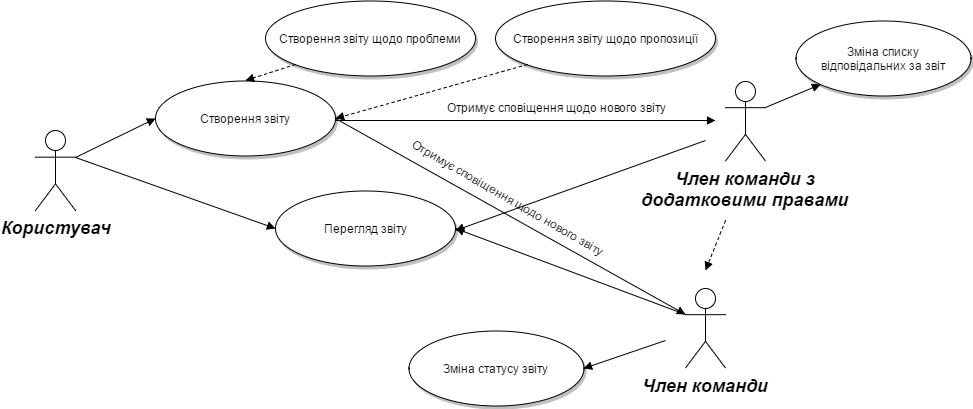
\includegraphics[width=1\textwidth]{diagram_usecase_1}
\caption{Механізму роботи зі звітами у вигляді діаграми прецедентів}
\end{figure}

\subsection{Формулювання та аналіз вимог за допомогою діаграми діяльності}
\begin{figure}[H]
\centering
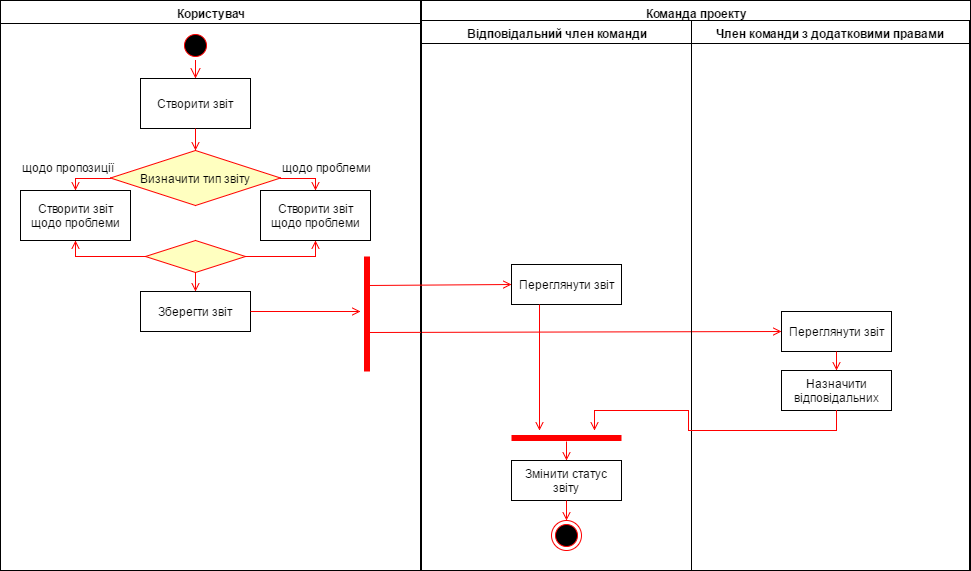
\includegraphics[width=1\textwidth]{diagram_activity_1}
\caption{Механізм роботи зі звітами у вигляді діаграми діяльності}
\end{figure}

% TODO: implement this

% \subsection{Аналіз вимог за допомогою діаграми послідовності}

% \subsection{Аналіз вимог за допомогою діаграми комунікації}

% \section{Визначення поведінки об'єктів багтрекінгової системи}

\end{document}